\documentclass[12pt]{article}

% TODO: Review grammar, spelling, and consistency.
% TODO: Comment and modularize the code.
% TODO: Check code consistency.
% TODO: Add more spacing between lines, table cells, and others.

\usepackage[a4paper, hmargin=0.8in, vmargin=1.2in]{geometry}
\usepackage{float} % For [H] placement specifier, which forces the figure/table to be placed exactly where it appears in the code.
\usepackage{setspace} % For line spacing

\usepackage{amsmath}
\usepackage{amssymb}
\usepackage{steinmetz} % For phasor notation
\usepackage{siunitx}

\usepackage{circuitikz}

\renewcommand{\arraystretch}{1.5}  % 1.5x default vertical spacing in tables
\renewcommand{\figurename}{Fig}

\parindent 0pt
\sisetup{inter-unit-product=\ensuremath{{}\cdot{}}, detect-weight}

\begin{document}

\begin{center}
	\begin{LARGE}
		\textbf{Experiment 8 Report}

		\vspace{20pt}
		\textbf{Verification of KCL for AC Circuits}
	\end{LARGE}
\end{center}

\begin{Large}
	\vspace{40pt}
	\textbf{Course No: EEE 164}
\end{Large}

\begin{large}
	\vspace{40pt}
	\begin{minipage}{0.48\textwidth}
		Experiment No: 08\\
		Department: CSE\\
		Section: B2
	\end{minipage}
	\hfill
	\begin{minipage}{0.48\textwidth}
		\textbf{Student ID: 2405103}\\
		Name: Kazi Md. Raiyan\\
		Lab Group No: 03
	\end{minipage}

	\vfill

	\begin{minipage}[t]{0.48\textwidth}
		Date of Performance: 12.07.2025\\
		Date of Submission: % TODO: Add submission date.
	\end{minipage}
	\hfill
	\begin{minipage}[t]{0.48\textwidth}
		\textbf{Partners' Student ID:}\\
		2405104\\
		2405105\\
		2405106\\
		2405107\\
		2405108
	\end{minipage}
	\vspace{80pt}

	\newpage
	\section{Objectives}
	This experiment is designed to:
	\begin{itemize}
		\item Verify KCL for AC circuits.
	\end{itemize}

	Upon successful completion of this experiment, we should be able to:
	\begin{itemize}
		\item Construct RLC circuits.
		\item Understand the validity of analytical methods used in theory.
	\end{itemize}

	\section{Apparatus}
	\begin{enumerate}
		\item Function generator
		\item Oscilloscope
		\item Multimeter
		\item Two $ \SI{100}{\ohm} $ resistors
		\item One $ \SI{120}{\ohm} $ resistor
		\item One $ \SI{1}{\micro\farad} $ capacitor
		\item Breadboard
	\end{enumerate}
	The ratings of the equipment supplied were checked.

	\section{Experimental Setup}
	\begin{figure}[H]
		\centering
		\begin{circuitikz}[american, voltage shift=0.8]
			% Source branch
			\draw (0,0) to[vsourcesin, v_={$ \textbf{V} = 5\phase{0^\circ} \SI{}{\V} $}] (0,-5);

			% Resistor and capacitor branches
			\draw
			(0,0) to[R, l={$ R_1 = \SI{98.5}{\ohm} $ }, i>^=$ \mathbf{I} $, v_=$ \mathbf{V}_{R_1} $] (4,0) -- (8,0);
			\draw (4,0) to[R, l={$ R_3 = \SI{119}{\ohm} $}, i>^=$ \mathbf{I}_2 $, v_=$ \mathbf{V}_{R_3} $] (4,-5);
			\draw (8,0) to[R, l={$ R_2 = \SI{99}{\ohm} $}, i>^=$ \mathbf{I}_1 $, v_=$ \mathbf{V}_{R_2} $] (8,-3) to[C, l={$ C = \SI{1}{\micro\farad} $}] (8,-5);
			\draw (0,-5) -- (8,-5);
			\draw (0,-5) node[ground] {};

			% Oscilloscope channels
			\draw (0,0) to[short, -*] (-1,1) node[left] {Channel 1};
			\draw (8,0) to[short, -*] (9,1) node[right] {Channel 2};
			\draw (0, -5) to[short, -*] (-1,-6) node[left] {Ref};
		\end{circuitikz}
		\caption{Circuit 1}
		\label{fig:circuit1}
	\end{figure}
	\begin{figure}[H]
		\centering
		\begin{circuitikz}[american]
			% Source branch
			\draw (0,0) to[vsourcesin, v_={$ \mathbf{V} = 5\phase{0^\circ} \SI{}{\V} $}] (0,-5);

			% Resistor and capacitor branches
			\draw (0,0) to[short, i>^=$ \mathbf{I} $] (4,0) -- (8,0);
			\draw (4,0) to[R, l={$ R_3 = \SI{119}{\ohm} $}, i>^=$ \mathbf{I}_2 $, v_=$ \mathbf{V}_{R_3} $] (4,-5);
			\draw (8,0) to[R, l={$ R_2 = \SI{99}{\ohm} $}, i>^=$ \mathbf{I}_1 $, v_=$ \mathbf{V}_{R_2} $] (8,-3) to[C, l={$ C = \SI{1}{\micro\farad} $}] (8,-5);
			\draw (0,-5) to[R, l={$ R_1 = \SI{98.5}{\ohm} $}, v_<=$ \mathbf{V}_{R_1} $] (4,-5) -- (8,-5);
			\draw (0,-5) node[ground] {};

			% Oscilloscope channels
			\draw (0,0) to[short, -*] (-1,1) node[left] {Channel 1};
			\draw (8,-5) to[short, -*] (9,-6) node[right] {Channel 2};
			\draw (0, -5) to[short, -*] (-1,-6) node[left] {Ref};
		\end{circuitikz}
		\caption{Circuit 2}
		\label{fig:circuit2}
	\end{figure}

	\section{Procedure}
	\begin{enumerate}
		\item The resistance of the resistors was measured with the help of the multimeter and the values were recorded.
		\item The frequency $ f $ of the function generator was set at $ \SI{1}{\kilo\hertz} $. The power source was not turned on yet.
		\item At first, circuit was setup as shown in Fig~\ref{fig:circuit1}.
		\item Then the magnitude and phase of the voltage $ \mathbf{V}_{R_3} $ were determined using the multimeter and the oscilloscope respectively.
		\item Then the phasor currents $ \mathbf{I}_1 = \mathbf{I}_{R_2} = \mathbf{I}_C = \dfrac{\mathbf{V}_{R_3}}{Z_{RC}} $ and $ \mathbf{I}_2 = \dfrac{\mathbf{V}_{R_3}}{R_3} $ were determined mathematically, where $ Z_{RC} $ is the equivalent impedance of $ R_2 $ and $ C $.
		\item Then the circuit was setup as shown in Fig~\ref{fig:circuit2}.
		\item Then the magnitude and phase of the voltage $ \mathbf{V}_{R_1} $ were determined using the multimeter and the oscilloscope respectively.
		\item Then the phasor current $ \mathbf{I} = \mathbf{I}_{R_1} = \dfrac{\mathbf{V}_{R_1}}{R_1} $ was determined mathematically.
		\item Then the phasor voltage $ \mathbf{V}_{R_2} $ was determined mathematically.
		\item The steps 3-9 were repeated for $ \SI{0.5}{\kilo\hertz} $ and $ \SI{2}{\kilo\hertz} $ source frequency.
		\item The phasor values of $ \mathbf{I} $, $ \mathbf{I}_1 $ and $ \mathbf{I}_2 $ were determined theoretically for the three frequencies and compared to the experimentally found values.
	\end{enumerate}

	\section{Data Collection}
	\textbf{Measurements:}\\
	\begin{minipage}{0.3\textwidth}
		$ R_1 = \SI{98.5}{\ohm} $
	\end{minipage}
	\hfill
	\begin{minipage}{0.3\textwidth}
		$ R_2 = \SI{99}{\ohm} $
	\end{minipage}
	\hfill
	\begin{minipage}{0.3\textwidth}
		$ R_3 = \SI{119}{\ohm} $
	\end{minipage}

	\vspace{20pt}
	\textbf{Table:}
	\begin{table}[H]
		\resizebox{\textwidth}{!}{
			\begin{tabular}{ |c|c|c|c|c|c|c|c| }
				\hline
				$ f (\SI{}{\kilo\hertz}) $ & $ \mathbf{V}_{R_2} (\SI{}{\V}) $ & $ \mathbf{V}_{R_3} (\SI{}{\V}) $ & $ \mathbf{I}_1 (\SI{}{\milli\A}) $ & $ \mathbf{I}_2 (\SI{}{\milli\A}) $ & $ \mathbf{V}_{R_1} (\SI{}{\V}) $ & $ \mathbf{I} (\SI{}{\milli\A}) $ & $ \mathbf{I}_1 + \mathbf{I}_2 (\SI{}{\milli\A}) $ \\
				\hline
				0.5                        & $ 0.55\phase{66.6^\circ} $       & $ 2.01\phase{-6.12^\circ} $      & $ 6.03\phase{66.6^\circ} $         & $ 16.89\phase{-6.12^\circ} $       & $ 1.89\phase{6.48^\circ} $       & $ 19.19\phase{6.48^\circ} $      & $ 19.55\phase{11.01^\circ} $                      \\
				\hline
				1                          & $ 0.82\phase{50.9^\circ} $       & $ 1.72\phase{-7.2^\circ} $       & $ 9.17\phase{50.9^\circ} $         & $ 14.45\phase{-7.2^\circ} $        & $ 2.02\phase{7.2^\circ} $        & $ 20.5\phase{7.2^\circ} $        & $ 20.8\phase{14.77^\circ} $                       \\
				\hline
				2                          & $ 1.02\phase{30.15^\circ} $      & $ 1.45\phase{-8.64^\circ} $      & $ 11.4\phase{30.15^\circ} $        & $ 12.18\phase{-8.66^\circ} $       & $ 2.09\phase{7.2^\circ} $        & $ 21.22\phase{7.2^\circ} $       & $ 22.24\phase{10.07^\circ} $                      \\
				\hline
			\end{tabular}
		}
		\caption{Experimental values}
		\label{tab:experimental_values}
	\end{table}

	\section{Report}
	\subsection{Theoretically calculate all the values written in the table.}
	{\setstretch{1.5}
		% 0.5 kHz
		\underline{For $ f = \SI{0.5}{\kilo\hertz} $:}\\
		$ \omega = 2 \pi f = \SI{3.141e3}{\radian\per\s} $\\
		$ Z_C = - \dfrac{1}{\omega C} j = -318.310 j \SI{}{\ohm} $\\
		$ \therefore Z_{eq} = R_1 + ({R_3}^{-1} + (R_2 + Z_C)^{-1})^{-1} = 199.076\phase{-8.75^\circ} \SI{}{\ohm} $\\
		$ \therefore \mathbf{I} = \dfrac{\mathbf{V}}{Z_{eq}} = 25.116\phase{8.75^\circ} \SI{}{\milli\A} $\\
		Now using the current divider rule:\\
		$ \mathbf{I}_1 = \dfrac{R_3}{R_3 + R_2 + Z_C} \mathbf{I} = 7.747\phase{64.34^\circ} \SI{}{\milli\A} $, and\\
		$ \mathbf{I}_2 = \dfrac{R_2 + Z_C}{R_3 + R_2 + Z_C} \mathbf{I} = 21.701\phase{-8.38^\circ} \SI{}{\milli\A} $\\
		$ \therefore \mathbf{V}_{R_1} = \mathbf{I} R_1 = 2.474\phase{8.75^\circ} \SI{}{\V} $\\
		$ \therefore \mathbf{V}_{R_2} = \mathbf{I_1} R_2 = 0.767\phase{64.34^\circ} \SI{}{\V} $\\
		$ \therefore \mathbf{V}_{R_3} = \mathbf{I_2} R_3 = 2.582\phase{-8.38^\circ} \SI{}{\V} $

		% 1 kHz
		\vspace{20pt}
		\underline{For $ f = \SI{1}{\kilo\hertz} $:}\\
		$ \omega = 2 \pi f = \SI{6.283e3}{\radian\per\s} $\\
		$ Z_C = - \dfrac{1}{\omega C} j = -159.155 j \SI{}{\ohm} $\\
		$ \therefore Z_{eq} = R_1 + ({R_3}^{-1} + (R_2 + Z_C)^{-1})^{-1} = 177.835\phase{-10.02^\circ} \SI{}{\ohm} $\\
		$ \therefore \mathbf{I} = \dfrac{\mathbf{V}}{Z_{eq}} = 28.116\phase{10.02^\circ} \SI{}{\milli\A} $\\
		Now using the current divider rule:\\
		$ \mathbf{I}_1 = \dfrac{R_3}{R_3 + R_2 + Z_C} \mathbf{I} = 12.396\phase{46.15^\circ} \SI{}{\milli\A} $, and\\
		$ \mathbf{I}_2 = \dfrac{R_2 + Z_C}{R_3 + R_2 + Z_C} \mathbf{I} = 19.524\phase{-11.97^\circ} \SI{}{\milli\A} $\\
		$ \therefore \mathbf{V}_{R_1} = \mathbf{I} R_1 = 2.769\phase{10.02^\circ} \SI{}{\V} $\\
		$ \therefore \mathbf{V}_{R_2} = \mathbf{I_1} R_2 = 1.227\phase{46.15^\circ} \SI{}{\V} $\\
		$ \therefore \mathbf{V}_{R_3} = \mathbf{I_2} R_3 = 2.323\phase{-11.97^\circ} \SI{}{\V} $

		% 2 kHz
		\vspace{20pt}
		\underline{For $ f = \SI{2}{\kilo\hertz} $:}\\
		$ \omega = 2 \pi f = \SI{1.257e4}{\radian\per\s} $\\
		$ Z_C = - \dfrac{1}{\omega C} j = -79.577 j \SI{}{\ohm} $\\
		$ \therefore Z_{eq} = R_1 + ({R_3}^{-1} + (R_2 + Z_C)^{-1})^{-1} = 161.54\phase{-7.44^\circ} \SI{}{\ohm} $\\
		$ \therefore \mathbf{I} = \dfrac{\mathbf{V}}{Z_{eq}} = 30.95\phase{7.44^\circ} \SI{}{\milli\A} $\\
		Now using the current divider rule:\\
		$ \mathbf{I}_1 = \dfrac{R_3}{R_3 + R_2 + Z_C} \mathbf{I} = 15.871\phase{27.50^\circ} \SI{}{\milli\A} $, and\\
		$ \mathbf{I}_2 = \dfrac{R_2 + Z_C}{R_3 + R_2 + Z_C} \mathbf{I} = 16.941\phase{-11.30^\circ} \SI{}{\milli\A} $\\
		$ \therefore \mathbf{V}_{R_1} = \mathbf{I} R_1 = 3.049\phase{7.44^\circ} \SI{}{\V} $\\
		$ \therefore \mathbf{V}_{R_2} = \mathbf{I_1} R_2 = 1.571\phase{27.50^\circ} \SI{}{\V} $\\
		$ \therefore \mathbf{V}_{R_3} = \mathbf{I_2} R_3 = 2.016\phase{-11.30^\circ} \SI{}{\V} $ \par}

	\vspace{20pt}
	\textbf{Table:}
	\begin{table}[H]
		\resizebox{\textwidth}{!}{
			\begin{tabular}{ |c|c|c|c|c|c|c| }
				\hline
				$ f (\SI{}{\kilo\hertz}) $ & $ \mathbf{I} (\SI{}{\milli\A}) $ & $ \mathbf{I}_1 (\SI{}{\milli\A}) $ & $ \mathbf{I}_2 (\SI{}{\milli\A}) $ & $ \mathbf{V}_{R_1} (\SI{}{\V}) $ & $ \mathbf{V}_{R_2} (\SI{}{\V}) $ & $ \mathbf{V}_{R_3} (\SI{}{\V}) $ \\
				\hline
				0.5                        & $ 25.116\phase{8.75^\circ} $     & $ 7.747\phase{64.34^\circ} $       & $ 21.701\phase{-8.38^\circ} $      & $ 2.474\phase{8.75^\circ} $      & $ 0.767\phase{64.34^\circ} $     & $ 2.582\phase{-8.38^\circ} $     \\
				\hline
				1                          & $ 28.116\phase{10.02^\circ} $    & $ 12.396\phase{46.15^\circ} $      & $ 19.524\phase{-11.97^\circ} $     & $ 2.769\phase{10.02^\circ} $     & $ 1.227\phase{46.15^\circ} $     & $ 2.323\phase{-11.97^\circ} $    \\
				\hline
				2                          & $ 30.95\phase{7.44^\circ} $      & $ 15.871\phase{27.50^\circ} $      & $ 16.941\phase{-11.30^\circ} $     & $ 3.049\phase{7.44^\circ} $      & $ 1.571\phase{27.50^\circ} $     & $ 2.016\phase{-11.30^\circ} $    \\
				\hline
			\end{tabular}
		}
		\caption{Theoretical values}
		\label{tab:theoretical_values}
	\end{table}

	\subsection{Draw the phasor diagrams for both the circuits of Fig~\ref{fig:circuit1} and Fig~\ref{fig:circuit2} for $ f = \SI{1}{\kilo\hertz} $ source frequency using the theoretical values. The diagrams should be drawn to scale on graph paper.}
	\begin{figure}[H]
		\centering
		\resizebox{0.6\textwidth}{!}{
			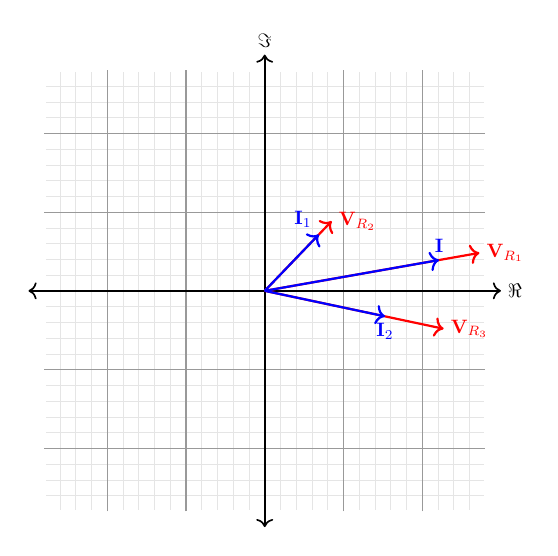
\begin{tikzpicture}[every node/.style={scale=0.7}]
				% Sub-grid
				\draw[very thin,color=gray!20] (-2.78,-2.78) grid[step=0.2] (2.78,2.78);

				% Grid
				\draw[thin,color=gray!80] (-2.8,-2.8) grid (2.8,2.8);

				% Axes
				\draw[<->, semithick] (-3,0) -- (3,0) node[right]{$ \Re $};
				\draw[<->, semithick] (0,-3) -- (0,3) node[above]{$ \Im $};

				% Voltage phasors
				\draw[->, red, thick] (0,0) -- (10.02:2.769) node[right]{$ \mathbf{V}_{R_1} $}; % V_R1
				\draw[->, red, thick] (0,0) -- (46.15:1.227) node[right]{$ \mathbf{V}_{R_2} $}; % V_R2
				\draw[->, red, thick] (0,0) -- (-11.97:2.323) node[right]{$ \mathbf{V}_{R_3} $}; % V_R3

				% Current phasors
				\draw[->, blue, thick, scale=0.08] (0,0) -- (10.02:28.116) node[above]{$ \mathbf{I} $}; % I
				\draw[->, blue, thick, scale=0.08] (0,0) -- (46.15:12.396) node[above left]{$ \mathbf{I}_1 $}; % I1
				\draw[->, blue, thick, scale=0.08] (0,0) -- (-11.97:19.524) node[below]{$ \mathbf{I}_2 $}; % I2
			\end{tikzpicture}
		}
		\caption{Phasor Diagram for Circuit 1 and Circuit 2 at $ f = \SI{1}{\kilo\hertz} $}
		\label{fig:phasor_diagram1}
	\end{figure}
	The phasor diagram for Circuit 1 and Circuit 2 is the same, because the circuits are essentially the same.

	\subsection{From the phasor diagram, express the voltages and the currents as phasors and compare those with the values in table~\ref{tab:experimental_values} for $ f = \SI{1}{\kilo\hertz} $.}
	From the phasor diagram, the voltages and currents at $ f = \SI{1}{\kilo\hertz} $ are:

	\begin{itemize}
		\item $ \mathbf{V}_{R_1} = 2.769\phase{10.02^\circ}~\SI{}{\V} $
		\item $ \mathbf{V}_{R_2} = 1.227\phase{46.15^\circ}~\SI{}{\V} $
		\item $ \mathbf{V}_{R_3} = 2.323\phase{-11.97^\circ}~\SI{}{\V} $
		\item $ \mathbf{I} = 28.116\phase{10.02^\circ}~\SI{}{\milli\A} $
		\item $ \mathbf{I}_1 = 12.396\phase{46.15^\circ}~\SI{}{\milli\A} $
		\item $ \mathbf{I}_2 = 19.524\phase{-11.97^\circ}~\SI{}{\milli\A} $
	\end{itemize}

	Comparing these theoretical phasor values with the experimental values in Table~\ref{tab:experimental_values} for $ f = \SI{1}{\kilo\hertz} $:

	\begin{table}[H]
		\resizebox{\textwidth}{!}{
			\begin{tabular}{|c|c|c|c|c|c|c|}
				\hline
				             & $ \mathbf{V}_{R_1}~(\SI{}{\V}) $ & $ \mathbf{V}_{R_2}~(\SI{}{\V}) $ & $ \mathbf{V}_{R_3}~(\SI{}{\V}) $ & $ \mathbf{I}~(\SI{}{\milli\A}) $ & $ \mathbf{I}_1~(\SI{}{\milli\A}) $ & $ \mathbf{I}_2~(\SI{}{\milli\A}) $ \\
				\hline
				Theoretical  & $ 2.769\phase{10.02^\circ} $     & $ 1.227\phase{46.15^\circ} $     & $ 2.323\phase{-11.97^\circ} $    & $ 28.116\phase{10.02^\circ} $    & $ 12.396\phase{46.15^\circ} $      & $ 19.524\phase{-11.97^\circ} $     \\
				\hline
				Experimental & $ 2.02\phase{7.2^\circ} $        & $ 0.82\phase{50.9^\circ} $       & $ 1.72\phase{-7.2^\circ} $       & $ 20.5\phase{7.2^\circ} $        & $ 9.17\phase{50.9^\circ} $         & $ 14.45\phase{-7.2^\circ} $        \\
				\hline
			\end{tabular}
		}
		\caption{Comparison of Theoretical and Experimental Values at $ f = \SI{1}{\kilo\hertz} $}
		\label{tab:exp_theory_comparison}
	\end{table}

	The experimental values are close to the theoretical values, with some differences due to measurement errors, non-ideal components, and faulty apparatus. Regardless, they confirm the validity of the theoretical analysis.

	\subsection{Show that the currents noted in table~\ref{tab:experimental_values} satisfy KCL for all three frequencies.}
	We can verify KCL by checking if the sum of the currents entering a node equals the sum of the currents leaving that node. Which means we need to check if $ \mathbf{I} = \mathbf{I}_1 + \mathbf{I}_2 $ holds true.

		{\setstretch{1.25}
			% 0.5 kHz
			\underline{For $ f = \SI{0.5}{\kilo\hertz} $:}\\
			From Table~\ref{tab:experimental_values}, we have:
			$ \mathbf{I} = 19.19\phase{6.48^\circ}~\SI{}{\milli\A} $\\
			$ \mathbf{I}_1 + \mathbf{I}_2 = 19.55\phase{11.01^\circ}~\SI{}{\milli\A} $\\
			$ \therefore \mathbf{I} \approx \mathbf{I}_1 + \mathbf{I}_2 $

			% 1 kHz
			\vspace{20pt}
			\underline{For $ f = \SI{1}{\kilo\hertz} $:}\\
			From Table~\ref{tab:experimental_values}, we have:
			$ \mathbf{I} = 20.5\phase{7.2^\circ}~\SI{}{\milli\A} $\\
			$ \mathbf{I}_1 + \mathbf{I}_2 = 20.8\phase{14.77^\circ}~\SI{}{\milli\A} $\\
			$ \therefore \mathbf{I} \approx \mathbf{I}_1 + \mathbf{I}_2 $

			% 2 kHz
			\vspace{20pt}
			\underline{For $ f = \SI{2}{\kilo\hertz} $:}\\
			From Table~\ref{tab:experimental_values}, we have:
			$ \mathbf{I} = 21.22\phase{7.2^\circ}~\SI{}{\milli\A} $\\
			$ \mathbf{I}_1 + \mathbf{I}_2 = 22.24\phase{10.07^\circ}~\SI{}{\milli\A} $\\
			$ \therefore \mathbf{I} \approx \mathbf{I}_1 + \mathbf{I}_2 $ \par}

	It can be seen that the currents satisfy KCL for all three frequencies, as the sum of the currents entering the node is approximately equal to the sum of the currents leaving the node.

	\subsection{Explain why we couldn't measure all the voltages with the circuit shown in fig~\ref{fig:circuit1}. Why it was essential to setup the circuit shown in fig~\ref{fig:circuit2}?}
	If we were to measure the voltage $ \mathbf{V}_{R_1} $ with the circuit shown in Fig~\ref{fig:circuit1}, we would have needed to connect the channel 2 probe where the channel 1 probe is connected, and the channel 2 reference probe at node A as shown in Fig~\ref{fig:circuit3}. This would have caused a short circuit, as the reference probe is grounded by default in the oscilloscope. Therefore, the circuit would have altered and the voltage $ \mathbf{V}_{R_1} $ would not have been measured correctly.
	However, by setting up the circuit shown in Fig~\ref{fig:circuit2}, we changed the position of $ R_1 $ effectively not changing the circuit, but allowing us to measure $ \mathbf{V}_{R_1} $ without causing a short circuit. This is why, it was essential to setup the circuit shown in Fig~\ref{fig:circuit2}.

	\begin{figure}[H]
		\centering
		\begin{circuitikz}[american, voltage shift=0.8]
			% Source branch
			\draw (0,0) to[vsourcesin, v_={$ \textbf{V} = 5\phase{0^\circ} \SI{}{\V} $}] (0,-5);
			
			% Resistor and capacitor branches
			\draw
			(0,0) to[R, l={$ R_1 = \SI{98.5}{\ohm} $ }, i>^=$ \mathbf{I} $, v_=$ \mathbf{V}_{R_1} $] (4,0) node[above right] {A} -- (8,0);
			\draw (4,0) to[R, l={$ R_3 = \SI{119}{\ohm} $}, i>^=$ \mathbf{I}_2 $, v_=$ \mathbf{V}_{R_3} $] (4,-5);
			\draw (8,0) to[R, l={$ R_2 = \SI{99}{\ohm} $}, i>^=$ \mathbf{I}_1 $, v_=$ \mathbf{V}_{R_2} $] (8,-3) to[C, l={$ C = \SI{1}{\micro\farad} $}] (8,-5);
			\draw (0,-5) -- (8,-5);
			\draw (0,-5) node[ground] {};

			% Oscilloscope channels
			\draw (0,0) to[short, -*] (-1,0) node[left] {Channel 1};
			\draw (0,0) to[short, -*] (0,1) node[left] {Channel 2};
			\draw (4,0) to[short, -*] (4,1) node[right] {Channel 2 Ref};
			\draw (0, -5) to[short, -*] (-1,-5) node[left] {Channel 1 Ref};
			
			% Short circuit
			\draw[red] (4,0) to[short, -, l_=Short Circuit] (0,-5);
		\end{circuitikz}
		\caption{Measuring $ \mathbf{V}_{R_1} $ with Circuit 1}
		\label{fig:circuit3}
	\end{figure}
\end{large}

\end{document}